\documentclass[tikz,border=2pt]{standalone}
\usepackage{tikz}
\usetikzlibrary{positioning}
\begin{document}
% Namikawa--Ueno type: I^*0-IV^*-t
% Target MRNC type: I^*0-IV^*-t
% Adapted from Tim Dokchitser picture: I^*_0\e({\it n})IV^*
% Parameter substitution: n -> t
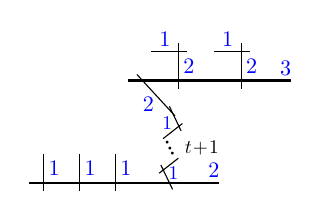
\begin{tikzpicture}[xscale=0.57,yscale=0.62]
\draw[thick,shorten >=2] (-1/3,0)--(121/30,0) node[inner sep=2pt,blue,above left,scale=0.8] {2};
\draw[shorten <=-3pt] (0,0)--node[inner sep=2pt,scale=0.8,blue,right] {1} (0,3/5);
\draw[shorten <=-3pt] (4/5,0)--node[inner sep=2pt,scale=0.8,blue,right] {1} (4/5,3/5);
\draw[shorten <=-3pt] (8/5,0)--node[inner sep=2pt,scale=0.8,blue,right] {1} (8/5,3/5);
\draw (14/5,0) 
    ++(0.07,-0.13)--++(-0.26,0.5)++(0.12,-0.19)  
    ++(0,0.02)
      node[blue,scale=0.7,inner sep=1,anchor=west]{1}
    ++(0,-0.02)
    ++(-0.16,0.02)--++(0.43,0.31)++(-0.13,0.07)  
    node{$\cdot$} ++(-0.06,0.12) node{$\cdot$}
    ++(-0.06,0.12) node{$\cdot$}++(0.17,-0.1)    node[auto,inner sep=5,scale=0.7,anchor=west]{$t\!+\!1$}
    ++(-0.26,0.19)--++(0.43,0.31)++(-0.18,0.04)   
    ++(0,-0.04)
      node[blue,scale=0.7,inner sep=1,anchor=east]{1}
    ++(0,0.04)
    ++(0.18,-0.04)++(-0.03,-0.15)--++(-0.26,0.5);
\draw[shorten <=-3pt, shorten >=-3pt] (14/5,3/2)--node[inner sep=2pt,scale=0.8,blue,below left=-1pt and -1pt] {2} (11/5,21/10);
\draw[thick,shorten >=2] (28/15,21/10)--(169/30,21/10) node[inner sep=2pt,blue,above left,scale=0.8] {3};
\draw[shorten <=-3pt, shorten >=-3pt] (3,21/10)--node[inner sep=2pt,scale=0.8,blue,right] {2} (3,27/10);
\draw[shorten <=-3pt] (3,27/10)--node[inner sep=2pt,scale=0.8,blue,above] {1} (12/5,27/10);
\draw[shorten <=-3pt, shorten >=-3pt] (22/5,21/10)--node[inner sep=2pt,scale=0.8,blue,right] {2} (22/5,27/10);
\draw[shorten <=-3pt] (22/5,27/10)--node[inner sep=2pt,scale=0.8,blue,above] {1} (19/5,27/10);
\end{tikzpicture}
\end{document}
